\documentclass[a4paper, 11pt]{article}
\title{Project: Automaten}
\author{Bas Van Assche, Tom Martens}
\usepackage[utf8]{inputenc}
\usepackage{hyperref}						%snelkoppeling in inhoudstafel
\usepackage{float}
\usepackage{graphicx} 						%foto's
\usepackage[usenames,dvipsnames]{color} 	%kleuren van woorden
\usepackage{url}
\hypersetup{
	colorlinks,
	citecolor=black,
	filecolor=black,
	linkcolor=black,
	urlcolor=black
}

\usepackage[dutch]{babel}
\usepackage[parfill]{parskip}
\usepackage[plain]{fancyref}
\usepackage[dvipsnames]{xcolor}
\usepackage{xspace}
\usepackage{amsmath}
\usepackage{amssymb}
\usepackage{mathtools}

\setlength{\textwidth}{0.75\paperwidth}
\setlength{\oddsidemargin}{0cm}
\setlength{\marginparwidth}{0cm}
\setlength{\marginparsep}{0cm}
\setlength{\voffset}{-2cm}
\setlength{\textheight}{700pt}


%%%%%%%%%%%%%%%%%%%%%%%%%%%%%%%

%%%%%%%%%%%%%%%%%%%%%%%%%%%%%%%


%header and footer
\usepackage{fancyhdr}
\pagestyle{fancy}
\lhead{Project: Automaten}
%header and footer

\begin{document}
	\maketitle
	\tableofcontents
	\newpage
	\section{Inleiding}
		Dit is een kort verlag waarin we bespreken hoe we alles hebben geïmplementeerd, wie welke onderdelen uitgevoerd heeft en welke problemen we zijn tegengekomen en hoe we die hebben aangepakt.
	
	\section{Structuur implementatie en beschrijving klassen}
		\textbf{Class Automaton:}
		Dit is de implementatie van de automaat zelf. Op deze automaat kan een intersectie met een andere automaat uitgevoerd worden en het kortste geaccepteerde pad of het kortste niet geaccepteerde pad kan gezocht worden. Een automaat wordt voorgesteld door een verzameling van States, finishstates en een startstate. Met de functies addEdge, addFinish en setStart wordt de automaat opgebouwd.
		
		\textbf{Class State:}
		Een State heeft een label en een lijst met Edges die vertrekken vanuit de state. Met de functie getEdgesStartingFromHere() kan men de lijst met Edges opvragen.
		
		\textbf{Class Edge:}
		Deze klasse stelt een edge voor uit de automaat met een start-state, een finish-state en een symbool.
		
		\textbf{Class AutomatonParser:}
		Deze klasse kan van een automaat inlezen uit een bestand en die automaat kan dan ook opgevraagd worden.
		
		\textbf{Class Level0:}
		Bij level 0 wordt het kortste pad van een automaat gegeven en indien er geen pad is wordt er “null” gegeven.
		
		\textbf{Class Level1:}
		Bij level 1 wordt het kortste pad van een automaat gegeven waarbij er 2 schatten gevonden zijn, waarbij er pas door een deur gegaan kan worden als een sleutel gevonden is en waarbij er onmiddellijk in de rivier gegaan moet worden als men langs de draak gaat wanneer men geen zwaard heeft.
		De nodige automaten wordt met de AutomatonParser ingelezen vanuit een file.
		
		\textbf{Class Level2:}
		Bij level 2 wordt het kortste pad van een automaat gegeven waarbij er 2 schatten gevonden zijn na het passeren van de laatste boog, waarbij er pas door een deur gegaan kan worden als een sleutel gevonden is en waarbij er onmiddellijk in de rivier gegaan moet worden als men langs de draak gaat wanneer men geen zwaard heeft.
		Ook hier worden de nodige automaten ingelezen vanuit een file.
		
		\section{Taakverdeling}
		De implementatie van de automaat is door Bas geïmplementeerd en de levels en de main klasse zijn door Tom geïmplementeerd.
		
		\section{Implementatie van levels}
		De levels zijn ontworpen om zo weinig mogelijk nodes te bevatten. Level 2 en 3 bestaan uit 3 verschillende automaten die vermenigvuldigd worden. Dus als we dan één node van een deelautomaat kunnen weghalen heeft dat een drastisch verschil op het totaal aantal nodes van de intersectie van het level met de adventure.
		
		Dit zijn de verschillende automaten die we gebruikt hebben voor de levels:
		
		\begin{figure}
			\centering
			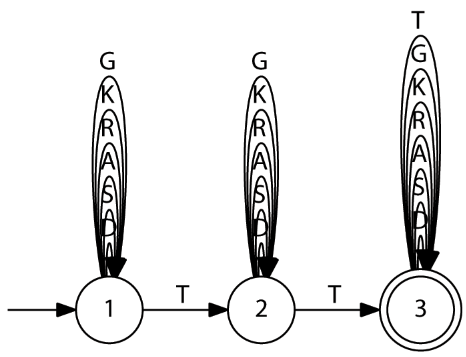
\includegraphics[width=0.4\linewidth]{2schatten}
			\caption{Minstens twee schatten vinden.}
			\label{fig:2schatten}
		\end{figure}
	
		
		\begin{figure}
			\centering
			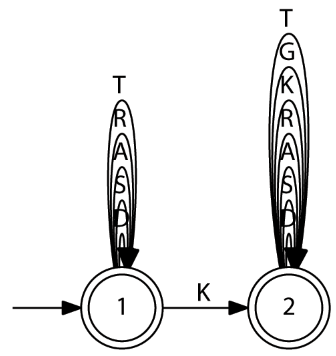
\includegraphics[width=0.3\linewidth]{sleutel}
			\caption{Sleutel vinden voor je door een deur kan.}
			\label{fig:sleutel}
		\end{figure}
	
		
		\begin{figure}
			\centering
			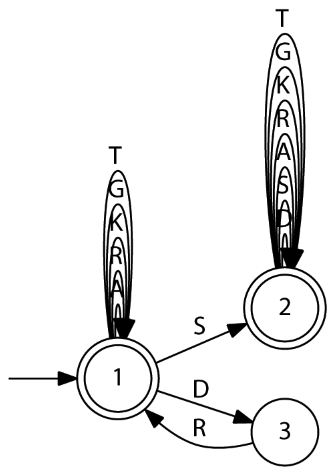
\includegraphics[width=0.3\linewidth]{draak}
			\caption{Na het passeren van een draak in het water springen als je geen zwaard hebt.}
			\label{fig:draak}
		\end{figure}
	
		
		\begin{figure}
			\centering
			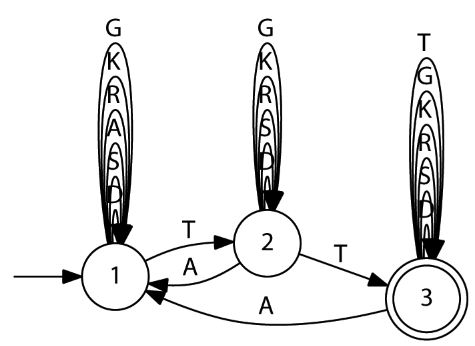
\includegraphics[width=0.4\linewidth]{boog}
			\caption{Bij het passeren van een boog speel je alle schatten kwijt.}
			\label{fig:boog}
		\end{figure}
		
		Als men in level 2 een boog passeert moet men alle schatten verliezen. We hebben dit gecombineerd met het zoeken van de twee schatten zoals in \fref{fig:boog} te zien is.
	
	\section{Problemen}
		We hadden gemerkt dat adventure 1 bij level 2 zeer lang moet rekenen. Eerst dachten we dat we een fout in onze implementatie hadden, maar na even na te denken bleek dat er enorm veel berekend moest worden omdat de automaat na intersectie meer dan 500 nodes groot is. We hebben daarna nog eens alle onderdelen van de levels overlopen op zoek naar een manier om het aantal nodes te kunnen verminderen. Uiteindelijk hebben we nog 2 nodes kunnen weghalen wat het totaal aantal nodes van adventure 1 op level 2 van 576 naar 288 bracht. Het doorlopen van level 2 is daardoor dus versneld, maar niet genoeg om snel tot een oplossing te komen voor adventure 1.
		Later merkte Bas op dat het berekenen van adventure 1 level 2 te lang duurt omdat het programma loops gaat maken, maar als er een pad is met een loop is er ook een korter pad zonder loop dus een node mag niet tweemaal voorkomen in één pad. Nadat Bas de implementatie van getShortestExample heeft aangepast ging de berekening zoveel sneller dat adventure 1 level 2 bijna onmiddellijk een oplossing geeft.
	
	
	
	
	
	
	
	
	
	
	
\end{document}